% High Bandwidth Low Latency Communication with SPI Devices Controlled by PIC32
\documentclass{beamer}
\usetheme{Warsaw}
\usecolortheme{dolphin}
\usefonttheme{professionalfonts}
\setbeamertemplate{footline}[frame number]
\setbeamertemplate{headline}{}

\usepackage[utf8]{inputenc}
\usepackage{graphicx}
\usepackage{tikz}
\usetikzlibrary{arrows.meta, positioning, fit}
\graphicspath{{../images/}{./images/}}

\title[HBLL SPI on PIC32]{High Bandwidth Low Latency Communication with SPI Devices Controlled by PIC32}
\subtitle{Bridging High-Speed Peripherals with External SRAM Buffers}
\author{Arturo Salinas and Alexander Xhemo}
%\institute{Univeristy of Connecticut}[ECE 3411 – Fall 2025]
\date{\today}

\begin{document}

% =====================
\begin{frame}
  \titlepage
\end{frame}

\begin{frame}{Outline}
  \tableofcontents
\end{frame}

\section{Project Overview}
\begin{frame}{Project Overview}
\begin{itemize}
  \item \textbf{Problem:} OV7670 camera outputs 8-bit parallel pixel data at \textbf{10–48 MHz}, while PIC32 runs at \textbf{40 MHz} and cannot sample/store 8 pins every few cycles without overrun.
  \item \textbf{Idea:} Use \textbf{8× 23LC1024 SPI SRAM} devices as a high-speed \textbf{parallel buffer} to absorb camera bursts, then \textbf{read out serially} via PIC32 at MCU pace.
  \item \textbf{Pipeline:} Target (camera) $\rightarrow$ SRAM (parallel write) $\rightarrow$ PIC32 (SPI read) $\rightarrow$ PC (UART $\rightarrow$ Python viewer).
  \item \textbf{Outcome:} Aligned frames captured; verified Y (luma) ordering and data integrity; color conversion needs further tuning.
\end{itemize}
\end{frame}

\section{Project Objectives \& Diagram}
\begin{frame}{Project Objectives}
\begin{enumerate}
  \item Capture a full CIF frame from OV7670 without MCU-cycle loss.
  \item Buffer high-rate parallel data directly into SRAM with minimal CPU intervention.
  \item Read buffered data back over SPI and stream to PC.
  \item Demonstrate low-latency control and high-bandwidth ingestion.
\end{enumerate}
\end{frame}

\section{High Level Diagram}
\begin{frame}{System Diagram}
  \begin{figure}[H]
    \centering
    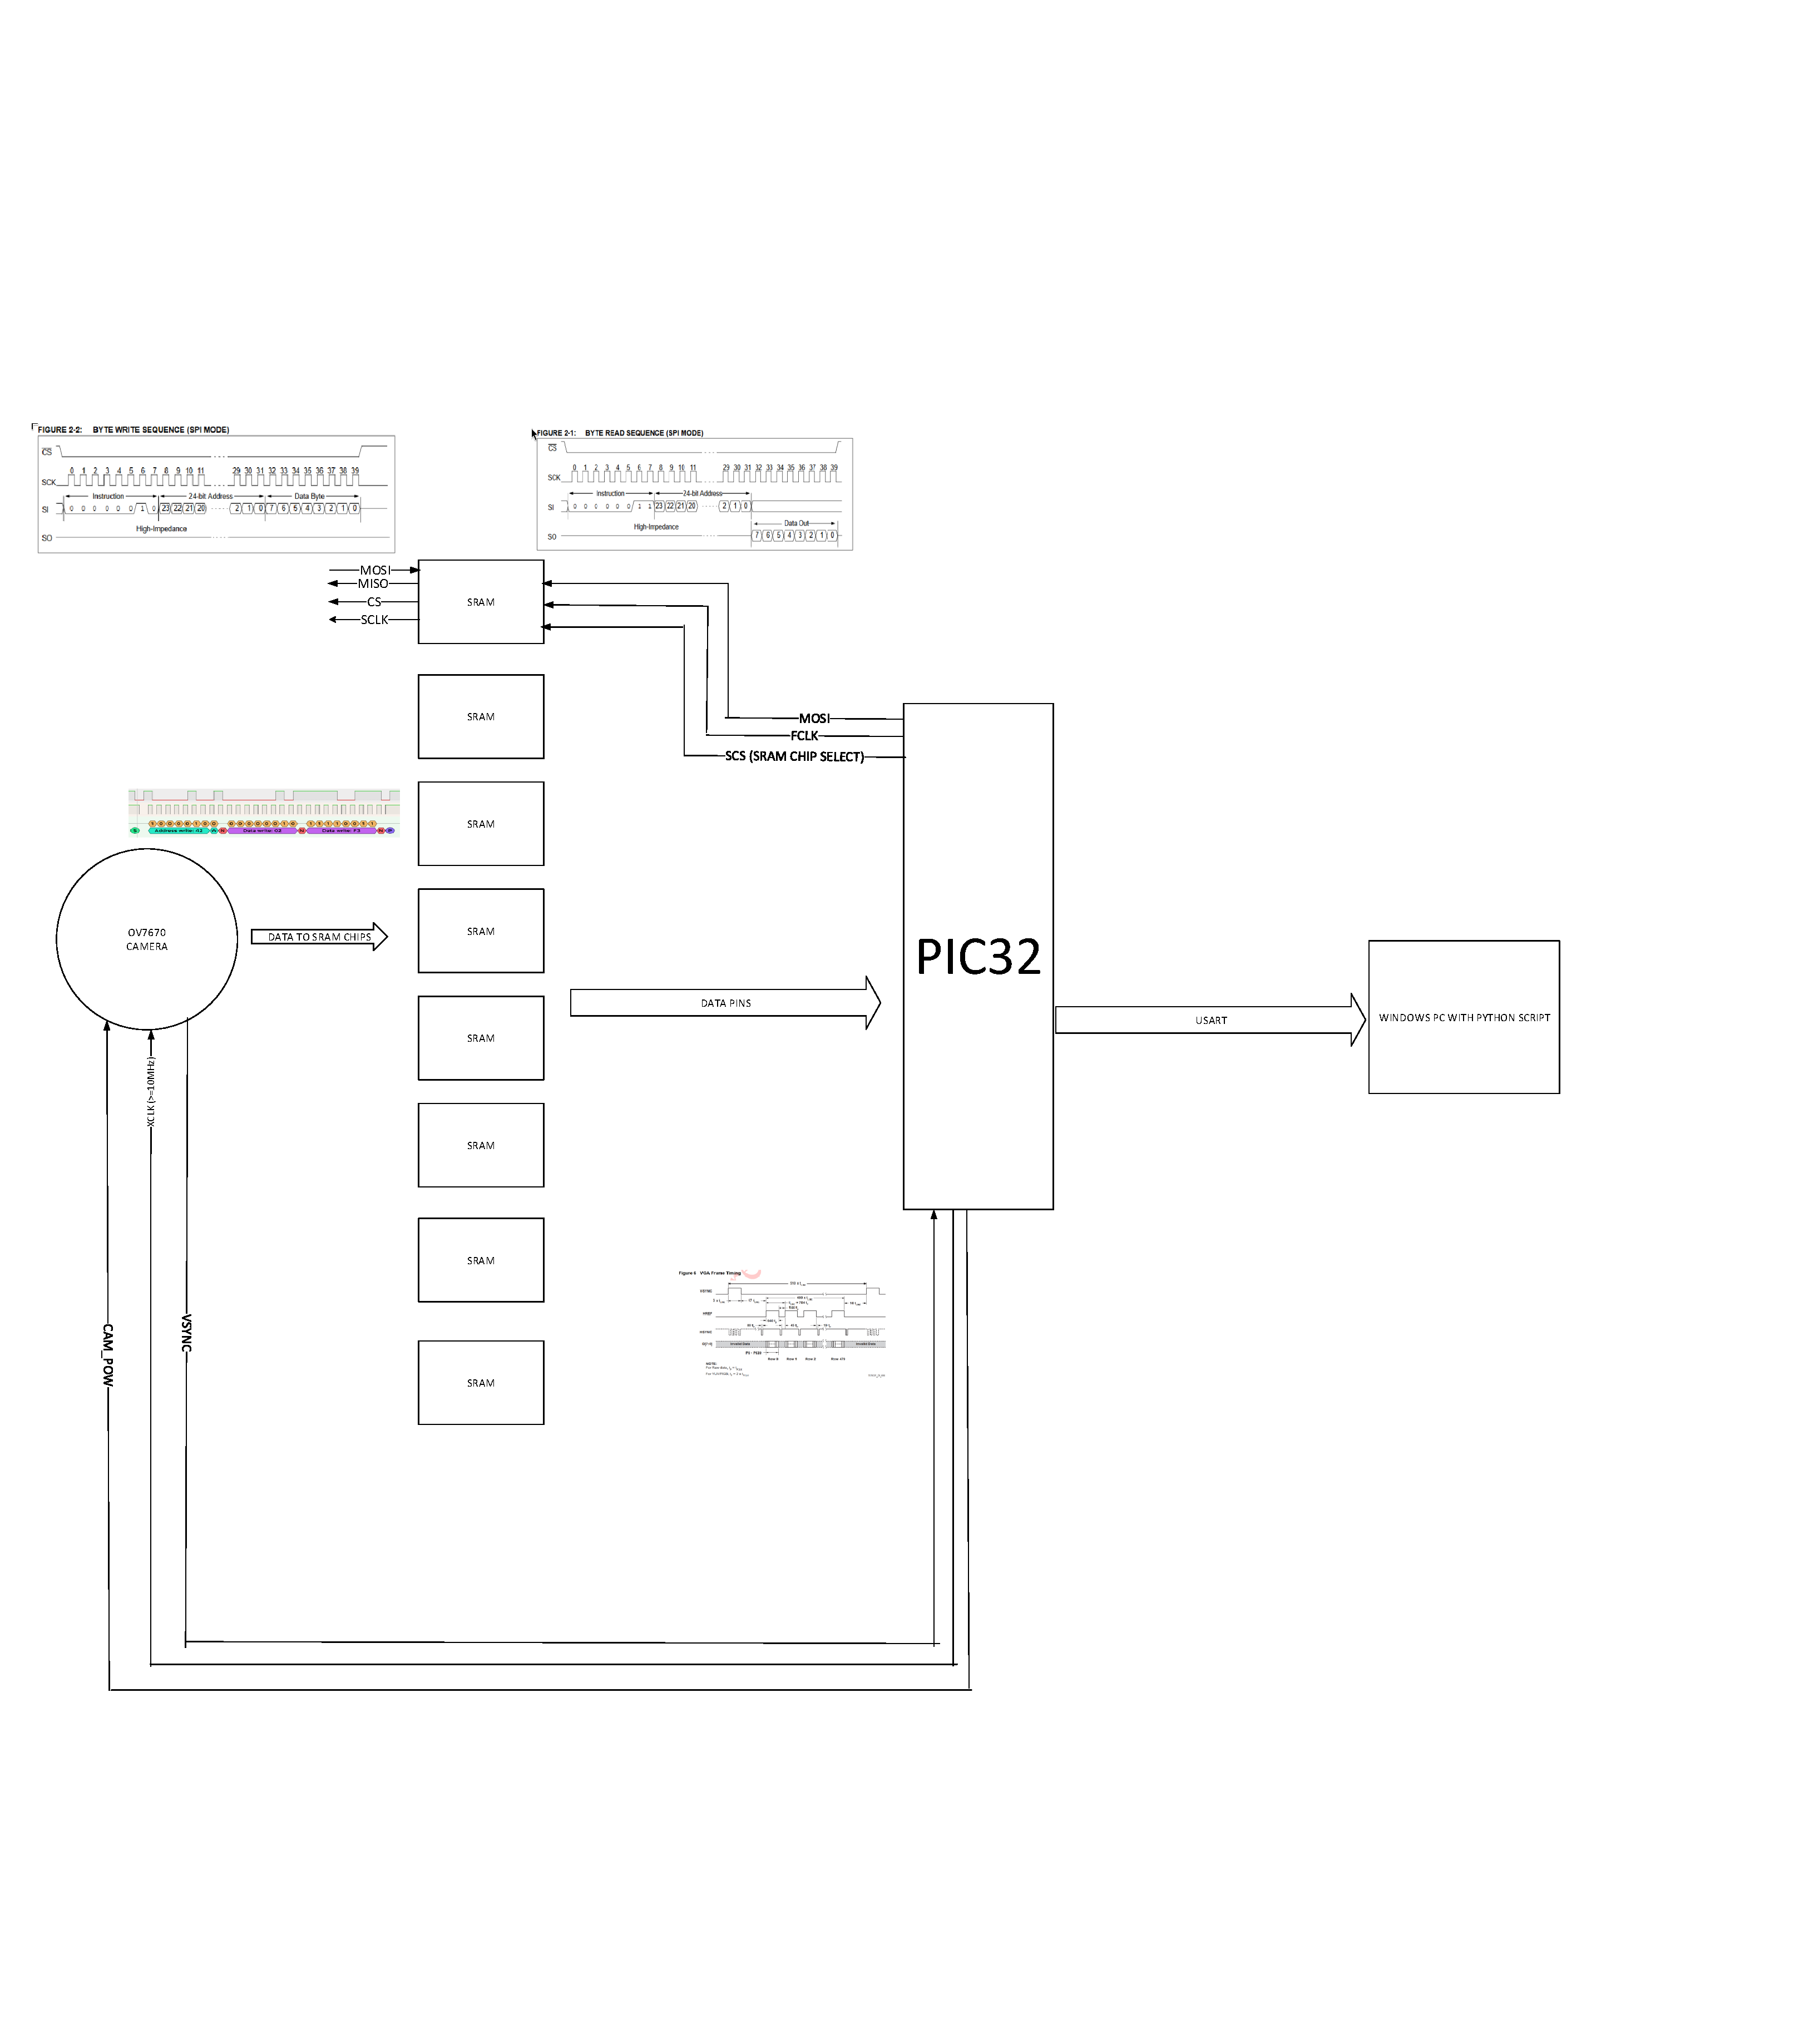
\includegraphics[width=0.65\textwidth]{SystemDiagram.pdf}
  \end{figure}
\end{frame}

\section{Hardware Components Used}
\begin{frame}{Hardware Components Used}
\begin{itemize}
  \item \textbf{PIC32} MCU at 40 MHz (SPI, UART, Output Compare for XCLK, GPIO).
  \item \textbf{OV7670 Camera}: 8-bit parallel data, SCCB configuration.
  \item \textbf{8 × 23LC1024 SPI SRAM}: parallelized as byte-wide buffer.
  \item \textbf{Glue Logic}: CS gating, clock selection (FCLK vs. PCLK), diode OR for MOSI lines, pull-downs.
  \item \textbf{Test Equipment}: Function generator (10 MHz XCLK), oscilloscope/logic analyzer.
\end{itemize}
\end{frame}

\section{Software Features}
\begin{frame}{Software Features}
  \begin{columns}
    \column{0.48\textwidth}
\begin{itemize}
  \item \textbf{Initialization}: Configure pins; generate XCLK (10 MHz) using Output Compare; set SCCB (I\textsuperscript{2}C-like) for camera registers.
  \item \textbf{Phase-Split Transaction}:
        \begin{itemize}
          \item \textit{P1 (PIC $\rightarrow$ SRAM)}: Drop CS, send \texttt{WRITE} + 24-bit address via MOSI/FCLK.
          \item \textit{P2 (Camera $\rightarrow$ SRAM)}: Camera drives D[0:7]; SRAM clocks on PCLK when HREF=1; CS held by logic until VSYNC rises.
        \end{itemize}
\end{itemize}
\column{0.48\textwidth}
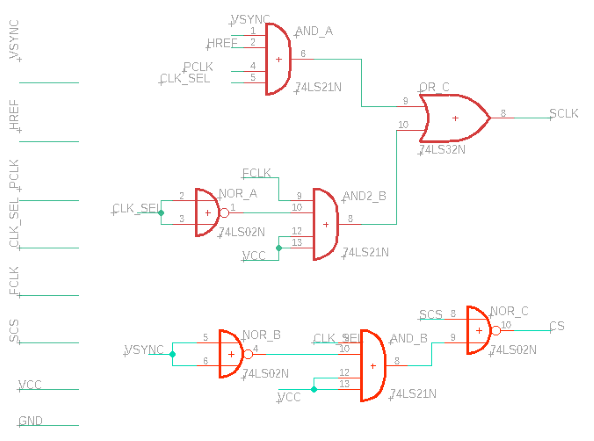
\includegraphics[width=\textwidth]{ControlClockHardware.png}
\end{columns}
\end{frame}

\begin{frame}{Software Features Cont.}
  \begin{columns}
    \column{0.48\textwidth}
    \begin{figure}[H]
      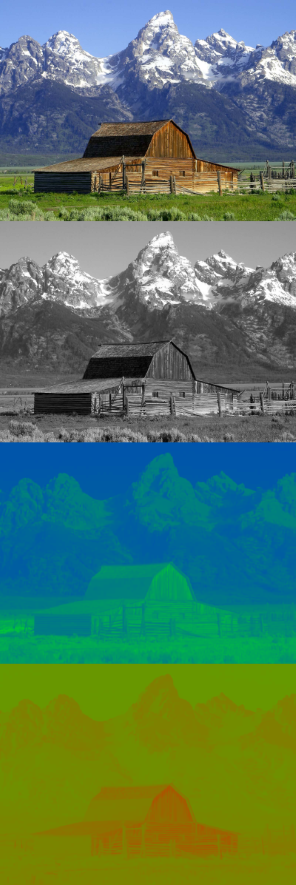
\includegraphics[width=\textwidth]{Barn-yuv.png}
    \end{figure}
    \column{0.48\textwidth}
      \begin{itemize}
      \item \textbf{Readout}: PIC32 issues \texttt{READ}; SPI-clocks bytes out of SRAM, forwards via UART to PC.
      \item \textbf{PC-side}: Python reconstructs image; attempts YUV$\rightarrow$RGB conversions; grayscale/Y channel validated.
      \end{itemize}
  \end{columns}
\end{frame}

\section{Microcontroller Peripherals}
\begin{frame}{Microcontroller Peripherals}
  \begin{columns}
    \column{0.48\textwidth}
    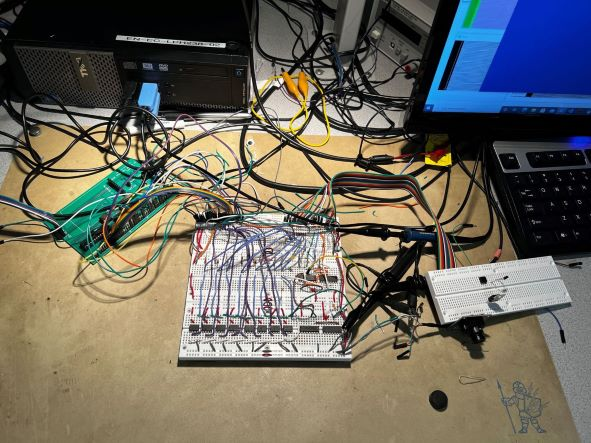
\includegraphics[width=\textwidth]{whole_project.jpg}

    \column{0.48\textwidth}
    \begin{itemize}
  \item \textbf{SPI}: Commanding SRAMs; sequential read/write.
  \item \textbf{UART}: Stream image bytes to host PC.
  \item \textbf{Output Compare (OC)}: Generate stable 10 MHz XCLK for camera.
  \item \textbf{GPIO}: VSYNC/HREF/PCLK sensing, SCS/CLK\_SEL/FCLK control, PORTY data capture.
  \item \textbf{SCCB (I\textsuperscript{2}C-like)}: Camera register programming (e.g., \texttt{COM7} reset/config).
    \end{itemize}
  \end{columns}
\end{frame}

\section{Results}
\begin{frame}{Results (Highlights)}
  \begin{columns}
    \column{0.48\textwidth}
\begin{itemize}
  \item \textbf{Acquisition}: Received full frames; VSYNC/HREF/PCLK timing honored.
  \item \textbf{Integrity}: Pixel alignment correct; grayscale (Y) images render as expected.
  \item \textbf{Throughput}: Parallel SRAM ingestion sustains camera rate with minimal CPU load.
  \item \textbf{Color}: YUV$\rightarrow$RGB conversion produced recognizable images; tuning needed for chroma interpretation.
\end{itemize}
\column{0.48\textwidth}
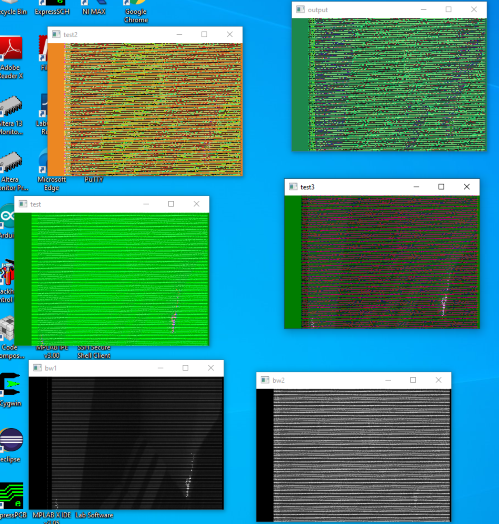
\includegraphics[width=\textwidth]{hoodie_pic.png}
\end{columns}
\end{frame}

\section{Lessons Learned}
\begin{frame}{Lessons Learned from the Project}
\begin{itemize}
  \item \textbf{Timing is king}: Edges (VSYNC/HREF/PCLK/SCK) and CS gating must be unambiguous. This just showed how the team learned about this specific interface.
  \item \textbf{Buffer-first architecture}: External SRAM decouples fast I/O from MCU constraints, many modern MCU's contain DRAM which can be utilized this way.
  \item \textbf{Tooling matters}: Logic analyzer + scope saved days of guesswork. In the field other timing tools can be used such as HDL Testbenches to verify timing constraints prior to hardware implementation.
  \item \textbf{Docs reality}: OV7670 documentation inconsistencies require empirical validation. This highlighted the teams inability to understand what the datasheet actually specifies.
  \item \textbf{Scalability}: Pattern applies to other wide, fast peripherals (ADCs, sensors), but can be improved.
\end{itemize}
\end{frame}
\section{Personal Opinions}
\begin{frame}{Opinions}
  \begin{itemize}
    \item \textbf{Reinventing the Wheel}: Other forms of buffers currently exist.
    \item \textbf{Difficulty with Synchronization}: Writing drivers for the timing could have been simplified using existing QSPI implementations
    \item \textbf{Reliance on Python}: The need to have a python script on the host windows PC greatly reduces the cool factor of this project.
    \end{itemize}
  \end{frame}

\section{Conclusion}
\begin{frame}{Conclusion \& Next Steps}
\begin{itemize}
  \item Demonstrated a practical \textbf{high-bandwidth, low-latency} bridge using \textbf{parallel SRAM} + \textbf{PIC32}.
  \item Verified frame capture correctness and robust readout path to PC.
  \item \textbf{Future work}: Better camera module; refine YUV$\rightarrow$RGB; add wireless link; DMA-assisted readout.
\end{itemize}
\end{frame}


\begin{frame}{Thank You}
\centering
Questions?
\end{frame}

\end{document}
